\chapter{Vergelijking}
\label{chap:vergelijking}

Dit hoofdstuk bekijkt hoe de mobiele HTML5 raamwerken zullen worden vergeleken.
Hoofdzakelijk zal dit gebeuren aan de hand van een \term{proof of concept}~(POC).
Deze wordt geïntroduceerd in sectie \ref{sec:vergelijking-poc} en zal hoofdzakelijk de gekozen vergelijkingscriteria in sectie \ref{sec:vergelijking-criteria} drijven.


\section{POC}
\label{sec:vergelijking-poc}
In sectie \ref{sec:vergelijking-poc-idee} wordt het idee van de gekozen POC besproken, waarna in sectie \ref{sec:vergelijking-poc-detail} de fases die door een werknemer worden uitgevoerd, gedetailleerd worden besproken.

\subsection{Idee}
\label{sec:vergelijking-poc-idee}

In samenspraak met Capgemini werd gekozen om een \term{proof of concept}~(POC) op te stellen.
Dit is een idee waarbij de uitvoerbaarheid in de verschillende raamwerken kan worden nagegaan.
Verschillende vergaderingen werden georganiseerd om tot een idee te komen dat vooral in de bedrijfswereld van toepassing is.
Het uiteindelijke idee is een applicatie die het mogelijk maakt voor werknemers om hun onkosten via hun mobiel apparaat door te sturen.

Het idee werd uitgewerkt door Capgemini en geleverd aan de auteurs als \term{mockup}.
Dit is een voorstelling van de applicatie als een reeks schermen zoals deze er zouden uitzien op een apparaat. 
Een voorbeeld van zo een scherm is te vinden op figuur~\ref{fig:poc}. 
De bedoeling is dat deze POC wordt uitgewerkt zowel voor smartphone als tablet, zowel voor Android als iOS, zowel voor staande als liggende apparaten en zowel voor online als offline gebruik.

\begin{figure}
  \centering
  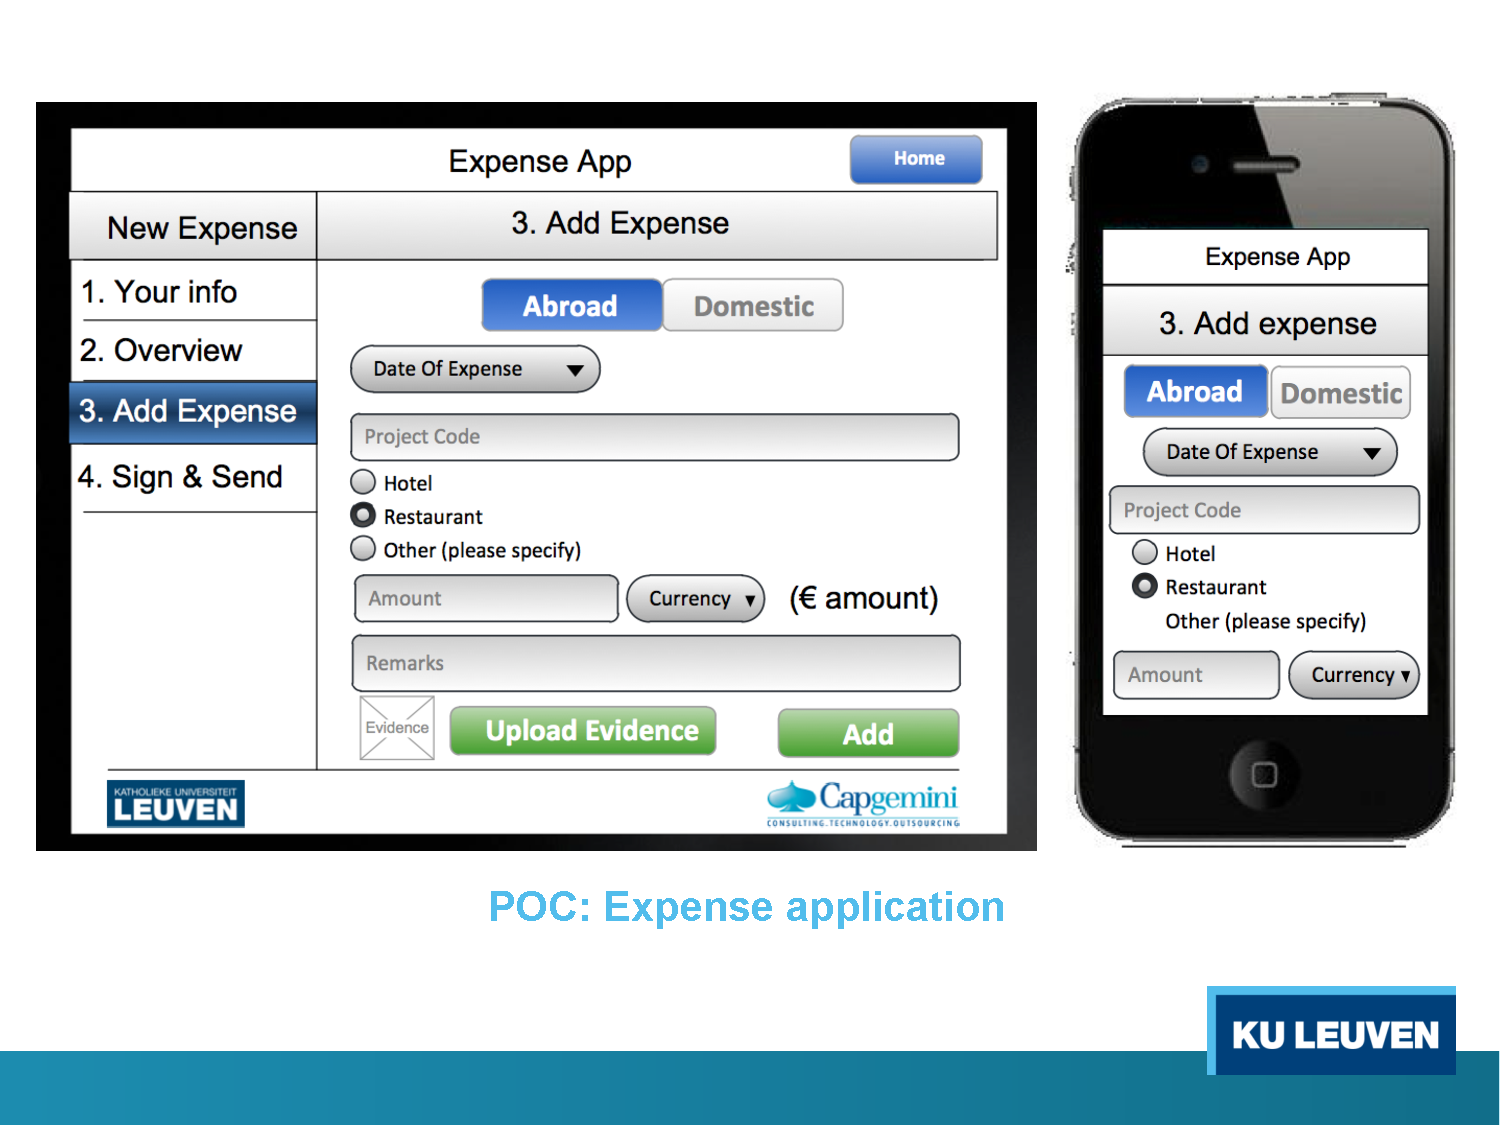
\includegraphics[trim=0cm 4cm 0cm 1.25cm,clip=true,height=7.5cm]{figuren/poc.pdf}
  \caption{POC bij het toevoegen van een nieuwe onkost met aan de linkerkant de weergave op een tablet en aan de rechterkant deze op een smartphone.}
  \label{fig:poc}
\end{figure}

\subsection{Aspecten}
\label{sec:vergelijking-poc-detail}

Een werknemer meldt zich eerst aan op de applicatie en kan daarna ofwel een nieuw onkostenformulier aanmaken of zijn doorgestuurde onkostenformulieren bekijken.
De term onkostenformulier is een groepering van meerdere onkosten met bijhorende bewijsstukken en de handtekening van de werknemer. 
Het aanmaken van een nieuw onkostenformulier verloopt in vier stappen.
Indien de werknemer al eerder begonnen was met het aanmaken van een formulier, zal hij worden gevraagd of hij verder wil gaan met dat formulier of met een nieuw formulier wil starten.

%Ik kreeg het gevoel dat de schrijfstijl veranderd.  Soms wordt er naar 'zijn', 'hij', ... verwezen,  dan weer is er de beschrijvende stijl met een verwijzing naar 'de werknemer`.. snapte? :) Tim: nee

\begin{enumerate}
\item De eerste stap is het bekijken en/of aanpassen van de persoonlijke informatie van de werknemer.
Bij het aanpassen van deze gegevens, zullen deze worden gevalideerd.
Indien deze validatie faalt, krijg de werknemer een dialoogvenster te zien met de reden tot falen.
Ook worden de foute velden rood gemarkeerd.

\item In de tweede stap kan de werknemer zijn toegevoegde onkosten aan het formulier bekijken.
In het begin is deze lijst leeg, tenzij hij eerder een formulier aan het invullen was (zie infra).
Indien deze lijst onkosten bevat, is het mogelijk om hierop te klikken en deze te bekijken. Aanpassen is niet mogelijk.

\item In stap drie kan een nieuwe onkost worden toegevoegd.
Dit kan ofwel een binnenlandse ofwel buitenlandse onkost zijn.
Voor beide dient een datum en projectcode te worden opgegeven.
De eerstgenoemde is een \term{datepicker} die teruggaat tot twee maanden in de tijd.
De laatstgenoemde bevat automatische aanvulling, maar de werknemer is niet verplicht om een projectcode uit de aanvulling te selecteren.
Daarnaast dient het type en bedrag van de onkost, alsook een bewijsstuk te worden opgegeven.
Bij een buitenlands onkost moet de munteenheid worden opgegeven, waarna de applicatie deze automatisch omvormt naar euro.
Het scherm voor het toevoegen van een buitenlandse onkost wordt getoond op figuur \ref{fig:poc}. 
Net zoals bij stap één geldt ook hier validatie op de formuliervelden.

\item In deze laatste stap dient een handtekening te worden geplaatst waarna het formulier kan worden doorgestuurd.
Indien de gebruiker offline werkt, zal deze worden opgeslagen op het toestel.
De werknemer kan het formulier opnieuw doorsturen zodra hij terug online is.

\end{enumerate}

Bij het bekijken van de doorgestuurde formulieren is het mogelijk om per formulier de bijhorende PDF te downloaden. 
Deze bevat een overzicht van de onkosten met bijhorende bewijsstukken, alsook de handtekening van de werknemer.

\section{Vergelijkingscriteria}
\label{sec:vergelijking-criteria}

In deze sectie zullen de criteria toelicht worden die zullen worden toegepast om de raamwerken te vergelijken.
In sectie \ref{sec:vergelijken-raamwerken} werden reeds technieken besproken die in de literatuur worden toegepast.
Elementen van deze technieken zullen terugkomen in onze methode om de raamwerken te evalueren.

%TODO passieve criteria, actieve criteria? De eerste zijn die van vorig hoofdstuk,  de laatste die nu volgen...
%Tim: dit moet zeker duidelijk naar voor komen, want dat is nogal belangrijk

Vijf grote criteria zullen worden gebruikt: gemeenschap (\ref{sec:vergelijking-gemeenschap}), productiviteit (\ref{sec:vergelijking-productiviteit}), gebruik (\ref{sec:vergelijking-gebruik}), ondersteuning (\ref{sec:vergelijking-ondersteuning}) en performantie (\ref{sec:vergelijking-performantie}). 
Elk raamwerk krijgt voor elk criterium een score. 
Deze scores zullen in een \term{spiderweb} worden ondergebracht.
Dit is een grafiek waar elke score in de overeenkomstige as met relatieve schaal wordt geplot.
Zoals hierboven vermeld zal een POC gebruikt worden bij de vergelijking.
De implementatie van deze POC zal het productiviteits-, gebruiks- en ondersteuningscriterium drijven.  
Dit komt omdat de auteurs ervan uitgaan dat de POC voldoende verschillende functionaliteit bevat om een goeie vergelijking te kunnen maken.
De score van performantie zal deels bepaald worden door de laadtijden van de POC.

\subsection{Gemeenschap}
\label{sec:vergelijking-gemeenschap}
De gemeenschap en populariteit van een raamwerk is in cijfers uit te drukken door gebruik te maken van sociale netwerken. 
Een tabel zal voorzien worden met in de kolommen het aantal volgers op Twitter, sterren en forkers van GitHub,  vragen op Stackoverflow en aantal \term{likes} van Facebook en de raamwerken in de rijen~\cite{Sarrafi2012a,Ayuso2012}. 
%TODO github nul geven als het niet beschikbaar is => verantwoorden dat het open source is
Ook de evolutie van deze data zal worden bekeken na een termijn van één maand.
Een grafiek van Google Trends, die het zoekvolume op Google uitzet per tijd, zal ook voor elk raamwerk worden toegevoegd.

De som van Twitter volgers ($T_r$), GitHub sterren ($S_r$), GitHub forkers ($F_r$), Stackoverflow vragen ($SO_r$) en Facebook \term{likes} ($FB_r$) vormt de score voor het gemeenschapscriteria:
\begin{equation}
  GM_r=T_r+S_r+F_r+SO_r+FB_r
  \label{eq:gemeenschap}
\end{equation}
met $r$ de verschillende raamwerken.

\paragraph{Motivatie}
TODO

%%%%%%%%%%%%%%%%%%%%%%%%%%%%%%%%%%%%%%%%%%%%%%%%%%%%%%%%%%%%%%%%%%
%%%%%%%%%%%%%%%%%%%%%%%%%%%%%%%%%%%%%%%%%%%%%%%%%%%%%%%%%%%%%%%%%%

\subsection{Productiviteit}
\label{sec:vergelijking-productiviteit}
De productiviteit moet een indicatie geven hoe lang het duurt om met het raamwerk vertrouwd te raken.
De auteurs zullen het raamwerk testen met een implementatie van de POC.
Er kan verondersteld worden dat de auteurs over een gemeenschappelijke technische achtergrond beschikken.
Elk zullen ze de POC in twee verschillende raamwerken maken,  daarnaast ook een extra loginscherm in twee andere raamwerken.
Tim Ameye maakt de POC in \jqm{} en \lungo{} en het loginscherm in \st{} en \kendo{}.
Sander Van Loock zal dan de POC in \st{} en \kendo{} maken en de loginschermen in \jqm{} en \lungo{}.
De tijd die nodig is om de volledige POC te implementeren is een indicatie voor de productiviteit. 
De implementatie van het loginscherm is een extra test.
Dit scherm bevat GI-elementen, validaties en \term{backend} integratie en kan dit dus als voldoende steekproef beschouwd worden om ervaring met een raamwerk te testen.
Het zal een indicatie geven hoe snel,  zonder al te veel voorkennis van het raamwerk,  één specifiek scherm kan opgeleverd worden.

De tijd die ieder nodig heeft om dit scherm te bouwen, geeft ook een indicatie van de nodige leertijd.


De som van de uren voor het implementeren van de POC ($t_{r,POC}$) en het loginscherm ($t_{r,login}$) vormt de score voor de productiviteit:
\begin{equation}
  PR_r = {t_{r,POC} + t_{r,login}}
  \label{eq:productiviteit}
\end{equation}
waar $r$ de verschillende raamwerken voorstellen.

\paragraph{Motivatie}
TODO

%%%%%%%%%%%%%%%%%%%%%%%%%%%%%%%%%%%%%%%%%%%%%%%%%%%%%%%%%%%%%%%%%%
%%%%%%%%%%%%%%%%%%%%%%%%%%%%%%%%%%%%%%%%%%%%%%%%%%%%%%%%%%%%%%%%%%

\subsection{Gebruik}
\label{sec:vergelijking-gebruik}
% Om het verschil in gebruik van de raamwerken te onderzoeken, zullen we steunen op de logboeken die we hebben bijgehouden tijdens het implementeren van de POC. 

% TODO Tim: ik zou onderstaande zin uit gebruik trekken, is ook relevant voor productiviteit en ondersteuning
%Sander: evt. alle assumpties ook met equations weergeven.  Dan kunnen we er altijd naar verwijzen als we ze nodig hebben?? Tim: ok voor mij
Men kan ervan uitgaat dat de POC alle relevante kenmerken bevat om de raamwerken zoveel mogelijk uit te buiten. 
Deze POC kan onderverdeeld worden in verschillende deelproblemen.
Deze deelproblemen worden als uitdaging aan het raamwerk voorgelegd.
Alle uitdagingen en sub uitdagingen zijn hieronder te vinden.

%TODO Tim: mooie oplossing hiervoor vinden, vragen aan Gonzalo? Sander: in appendix steken?
\begin{enumerate}[label*=U \arabic*.]
\item \label{challenge:formulieren}Formulieren
\begin{enumerate}[label*=\arabic*]
\item Maak formulieren met placeholders,  maar zonder labels
\item Gebruik tekst, numer en email als formulier types
\item Aangepaste \term{datepicker} met bereik van data
\item Aangepaste \term{datepicker} met enkel maand- en jaarveld
\item Wissen van een formulier
\end{enumerate}
\item \label{challenge:invullen}Invullen van een formulier
\begin{enumerate}[label*=\arabic*]
\item Vul formulierelementen met data
\item Maak elementen van het formulier \term{read-only}
\end{enumerate}
\item \label{challenge:validatie}Formulier validatie
\begin{enumerate}[label*=\arabic*]
\item Validatie regels voor verplichte,numer en email velden
\item Validatie regels voor eigen condities
\item Venster voor foutenboodschappen van ongeldige velden
\item Rode randen plaatsen rond ongeldige velden
\end{enumerate}
\item \label{challenge:handtekening}Handtekening
\begin{enumerate}[label*=\arabic*]
\item Teken een handtekening met vinger of pen
\end{enumerate}
\item \label{challenge:pdf}Toon PDF-bestand
\begin{enumerate}[label*=\arabic*]
\item Vraag een PDF-bestand op met POST parameters
\item Toon het PDF-bestand
\end{enumerate}
\item \label{challenge:afbeelding}Toevoegen van een afbeelding
\begin{enumerate}[label*=\arabic*]
\item Kies een afbeelding
\item Converteer de afbeelding met base64
\item Voorbeeld van de afbeelding
\end{enumerate}
\item \label{challenge:autoaanvullen}Autoaanvullen
\begin{enumerate}[label*=\arabic*]
\item Haal suggesties op gebaseerd op gebruikersinvoer
\item Toon suggesties in klikbare dropdownmenu
\end{enumerate}
\item \label{challenge:ajax}AJAX: tekst, JSON en XML
\begin{enumerate}[label*=\arabic*]
\item Haal tekst zonder opmaak op
\item Haal JSON data op en parse
\item Zend JSON data
\item Haal XML data op en parse
\end{enumerate}
\item \label{challenge:toestel}Toestel specifieke lay-out
\begin{enumerate}[label*=\arabic*]
\item Herkennen van smartphone en tablet
\item Toon het linker menu op een tablet
\item Schakel menu in bij smartphone
\end{enumerate}
\item \label{challenge:offline}Offline
\begin{enumerate}[label*=\arabic*]
\item Bewaar login gegevens
\item Bewaar niet verzonden onkosten
\item Maak de applicatie offline beschikbaar
\end{enumerate}
\item \label{challenge:laadscherm}Laadscherm en dialoog
\begin{enumerate}[label*=\arabic*]
\item Toon laadscherm
\item Toon dialoog
\end{enumerate}
\item \label{challenge:conversie}Data conversie
\begin{enumerate}[label*=\arabic*]
\item Conversie van munteenheid
\item Conversie van ids naar tekst	
\end{enumerate}
\item \label{challenge:lijsten}Lijsten
\begin{enumerate}[label*=\arabic*]
\item Laad data in lijst en stijl de elementen met een template
\item Klikbare lijst elementen met actie of link naar het record van het element
\item Sorting data
\end{enumerate}
\item \label{challenge:anatomie}Anatomie van een pagina
\begin{enumerate}[label*=\arabic*]
 \item Toon header,  footer en onderliggende header met titels en knoppen
 \item Tabbar
 \item Aanpasbaarheid van kleur van knoppen
 \end{enumerate}
\end{enumerate} 

De wijze waarop het raamwerk de uitdaging aangaat zal tot een score voor de uitdaging leiden.
In totaal zijn er drie gevallen.
De hoogste score wordt toegekend wanneer bepaalde functionaliteit reeds aangeboden wordt door het raamwerk. 
Een lagere score betekent dat een plug-in werd gezocht. 
Wanneer de code voor het overgrote deel zelf diende geschreven te worden of een hack noodzakelijk was, zal de laagste score worden toegekend.
Tabel \ref{tabel:scores-uitdagingen} toont de mogelijke scores $U_{r,i}$ van raamwerk $r$ en voor uitdaging $i$.
\begin{table}[h]	
  \centering
  \begin{tabular}{ll}
    \toprule
    \textbf{Score} & \textbf{Beoordelingscriteria}\\
    \midrule
    $U_{r,i} = 2$ & Ondersteund door het raamwerk\\
    $U_{r,i} = 1$ & Een plug-in is nodig\\
    $U_{r,i} = 0$ & Eigen implementatie of hack\\
    \bottomrule
  \end{tabular}
  \caption{Beoordeling uitdagingen gebruikscriterium}
  \label{tabel:scores-uitdagingen}
\end{table}
\begin{equation}
  GB_r = \sum_{i=1}^{14}{\left(U_{r,i}\right)}
  \label{eq:gebruik}
\end{equation}
met $r$ de verschillende raamwerken en $i$ de uitdagingen.

\paragraph{Motivatie}
TODO
%TODO Tim: uitleggen waarom we er 3 gekozen hebben en bv. niet de 4 van mij… 'omdat we raamwerken testen en niet pure HTML5/CSS3'

%%%%%%%%%%%%%%%%%%%%%%%%%%%%%%%%%%%%%%%%%%%%%%%%%%%%%%%%%%%%%%%%%%
%%%%%%%%%%%%%%%%%%%%%%%%%%%%%%%%%%%%%%%%%%%%%%%%%%%%%%%%%%%%%%%%%%

\subsection{Ondersteuning}
\label{sec:vergelijking-ondersteuning}
Dit criterium moet weergeven hoe goed het raamwerk verschillende toestellen met hun verschillende besturingssystemen ondersteund.
% TODO Tim: duidelijker uitleggen hoe dat zit met browser en OS, nu veel te kort tussen haakjes aangehaald
Enkel de standaard browser van het besturingssysteem (Android browser/Chrome en Safari) zal beschouwd worden.
Een \term{context} is één bepaalde configuratie van toestel, besturingssysteem en browser.
Alle uitdagingen die gebruikt zijn om het gebruikscriterium te testen komen ook hier van pas.
In elke context zullen de $14$ uitdagingen van de vorige sectie worden getest.
De correcte weergave en uitvoering van alle subuitdaging binnen een context bepaalt de score voor die context.
Deze score kan enkel $0$ of $1$ zijn om wille van respectievelijk een probleem of correcte uitvoering van de subuitdaging.
Per context zal ook de marktwaarde van het toestel in rekening worden gebracht om de meest gebruikte toestellen te bevoordelen.
De marktwaarde is afhankelijk van het besturingssysteem,  de versie van het besturingssysteem en de gebruikte mobiele browser.
%TODO Tim: gebruik van 'we'
Voor de marktwaarden wordt naar tabellen \ref{tabel:marktaandeel-ios-android} en \ref{tabel:marktaandeel-browsers} verwezen.
De formule voor de marktwaarde van een bepaalde context ziet er als volgt uit:
%TODO Sander: ook gewicht van device?
\begin{equation}
  G_c = G(BS_c)*G(BS_{c,v})*G(Browser_c)
 \label{eq:marktwaarde}
\end{equation}
met $G$ de functie die de marktwaarde teruggeeft.  
De marktwaarde voor Android en iOS ($G(BS_c)$) werd vermeld in sectie \ref{sec:mobiele-besturingssystemen}.
De relatieve marktwaarde van de versie van dat besturingssysteem ($G(BS_{c,v})$) kan gevonden worden in tabel \ref{tabel:marktaandeel-ios-android}.
De marktwaarde van mobiele webbrowsers ($G(Browser_c)$) kan gevonden worden in tabel \ref{tabel:marktaandeel-browsers}.

In tabel \ref{tabel:toestellen-hci} staan de verschillende contexten met hun marktwaarde weergegeven.

De gewogen som van de scores van de verschillende contexten bepaalt de score van het ondersteuningscriterium:
\begin{equation}
  O_r = \sum_{c=1}^{8}{\left(\sum_{i=1}^{13}U_{r,i}*G_c\right)}
  \label{eq:ondersteuning}
\end{equation}
met $r$ de verschillende raamwerken,  $c$ de verschillende contexten en $i$ de uitdagingen. 

% We zullen een scenario uitwerken waarbij we het gebruik van de POC doorlopen. 
% Dit scenario zullen we op een reeks van verschillende mobiele apparaten herhalen~\cite{Sarrafi2012a}. 
% Bij het mislukken van een stap in het scenario, zal een punt worden afgetrokken. 
% Hierdoor kunnen we een score bekomen hoe goed de applicatie, geïmplementeerd in een bepaald raamwerk, scoort op een bepaald apparaat. 
%De gebruikte apparaten araten aan het departement HCI.

%TODO Onderstaande wordt verplaatst naar hoofdstuk raamwerken
%Een kanttekening bij dit criterium is of het raamwerk ondersteunt de webapplicatie om te vormen tot een \term{native} applicatie. 
%Ook zal er gekeken worden of de \term{native look-and-feel} per platform door het raamwerk kan worden benaderd.

\begin{table}[h]
  \centering
  \begin{tabular}{lllll}
    \toprule
    \textbf{Toestel} & \textbf{Soort} &\textbf{Besturingssysteem} & \textbf{Browser} & \textbf{Marktwaarde ($G_d$)}\\
    \midrule
    HTCDesireZ & Smartphone & Android 2.3.3 & Android browser & $62586$\\ %75.0*45.6*18.30
    GalaxyTab & Tablet & Android 2.3.6 & Android browser & $62586$\\ %75.0*45.6*18.30
    GalaxyS & Smartphone  & Android 4.1.2 & Chrome & $1848.3$\\ %75.0*12.2*2.02
    Nexus 7 & Tablet & Android 4.2.1  & Chrome & $1848.3$\\ %75.0*2*2.02
    iPad1 WiFi & Tablet & iOS 5.1.1 & Mobile Safari & $15910.965$\\%14.9*17.5*61.02
    iPad3 4G WiFi & Tablet & iOS 6.0.1 & Mobile Safari & $36367.92$\\%14.9*40.0*61.02
    iPhone 3GS & Smartphone & iOS 6.0.1 & Mobile Safari & $36367.92$\\%14.9*40.0*61.02
    iPhone 4S & Smartphone & iOS 6.0.1 & Mobile Safari & $36367.92$\\%14.9*40.0*61.02
    \bottomrule
  \end{tabular}
  \caption{Beschikbare toestellen met hun besturingssysteem, browser en gewicht}
  \label{tabel:toestellen-hci}
\end{table}


\paragraph{Motivatie}
TODO

%%%%%%%%%%%%%%%%%%%%%%%%%%%%%%%%%%%%%%%%%%%%%%%%%%%%%%%%%%%%%%%%%%
%%%%%%%%%%%%%%%%%%%%%%%%%%%%%%%%%%%%%%%%%%%%%%%%%%%%%%%%%%%%%%%%%%

\subsection{Performantie}
\label{sec:vergelijking-performantie}
Dit criterium zal de laattijden van het raamwerk in rekening brengen.
De tijd die nodig is om één of meerder pagina's te laden zal bepaald worden met Google Page Speed~\cite{Morgan2011}. 
Hiervoor zullen verschillende testen worden uitgevoerd. 
Ten eerste zal de laadtijd van de volledig geïmplementeerde POC bekeken worden ($r_{r,POC}$). 
Daarnaast zullen geïsoleerde testen met het verzenden van een AJAX-request uitgevoerd worden ($r_{r,AJAX}$).
Daar wordt het effect van het versturen van een OPTION-\term{request} bekeken wanneer een verzoek naar een ander domeinen wordt gestuurd.
%TODO exacte info tests + extra info CORS zoeken

%Verdergaand op het versturen van requests zullen we kijken hoe lang het duurt vooraleer een expense daadwerkelijk verzonden is naar de backend.
Verder zijn er ook geïsoleerde testen met GI-elementen. 
Hier zal een \term{dummy} pagina voorzien worden 1000 knoppen van het raamwerk en bepaalt Google Page Speed de laadtijd ($r_{r,GI}$). 
%TODO exacte UI tests hier uitleggen
Als laatste zullen de loginschermen die in sectie \ref{sec:vergelijking-productiviteit} werden geïntroduceerd, worden gebruikt ($t_{r,login}$). 
De redenen waarom deze geïsoleerde applicatie wordt gebruiken is omdat ervan kan worden uitgegaan dat niet de volledige POC in ieder raamwerk zal kunnen worden geïmplementeerd. 
Dit is in tegenstelling tot dit scherm, waarbij exact het aantal lijnen code en bijhorende performantie kan worden vergeleken.

De formule voor het performantiecriterium wordt dan: 

\begin{equation}
  PE_r=r_{r,POC}+r_{r,AJAX}+r_{r,GI}+r_{r,login} 
  \label{eq:performantie}
\end{equation}
met $r$ de verschillende raamwerken.

\paragraph{Motivatie}
%TODO

%%%%%%%%%%%%%%%%%%%%%%%%%%%%%%%%%%%%%%%%%%%%%%%%%%%%%%%%%%%%%%%%%%
%%%%%%%%%%%%%%%%%%%%%%%%%%%%%%%%%%%%%%%%%%%%%%%%%%%%%%%%%%%%%%%%%%
